\chapter{Validation}

\section{Introduction}
After building our model inside the \textbf{OMNeT++} we can proceed with the simulation in order to analyze the quantities wich we are interested. First of all we will simulate the model in very simple cases in order to be sure it reproduces the system's behavior correctly. We decided to validate our model by \textit{removing randomness}. This choice allows us to do some easy computation by hand and to verify if the result of simulation is consistent with them. Our model will be considered a good replica of the system if it will pass all the \textit{validation tests}. During the validation we will use the first scheduler: \textbf{Round-Robin Frame Fill} because it generates simulation which are easier to analyze and to compare with analitical results.

\section{1\textsuperscript{st} test: fixed CQI, fixed \(\lambda\) rate, fixed packet size, 1 user}
In this test we just one \texttt{Mobile Station} connected to the antenna wich always generates the same CQI for each timeslot. Inside the \texttt{Web Server} the \(\lambda\) rate is fixed and also the packet size. This is a very simple system with deterministic arrivals and deterministic service demand. We can compute the traffic that \texttt{Web Server} sends to the antenna as 
\begin{equation} 
	th\textsubscript{in} = \frac{packetsize \times 8}{1/(1000\lambda)} \lbrack bps \rbrack 
\end{equation} 
If the system is in a stable state the output throughput and the input throughput must be equal. The maximum output throughput is the one we have by setting all parameters to maximum values. 
\begin{equation} 
	th\textsubscript{max} = \frac{\#RB \times RBsize\textsubscript{max} \times 8}{T\textsubscript{slot}} = \frac{25 \times 93 \times 8}{0.001} = 18.6 \textnormal{ Mbps}
\end{equation} 
We can derive very easily the \(\lambda\textsubscript{max}\) rate wich produces the max throughput allowed by antenna. 
\begin{equation}
	\lambda\textsubscript{max} = \frac{\#RB \times RBsize\textsubscript{max}}{1000 \times T\textsubscript{slot} \times packetsize\textsubscript{max}} = \frac{25 \times 93}{1000 \times 0.001 \times 75} = 31 \textnormal{ ms\textsuperscript{-1}} 
\end{equation}
For \( 0<\lambda<\lambda\textsubscript{max} \) the system is a stable state and so \(th\textsubscript{in} = th\textsubscript{out}\). For higher \(\lambda\) the FIFOQueue grows indefinitely because the frame is not able to carry as much data in a time slot.

Let's consider all the simulations with the following parameters:
\begin{itemize}
	\item \(\lambda \in \{1,2,\ldots,32\}\)
	\item \(packetsize=75\)
	\item \(CQI=15\)
\end{itemize}
  We can se in the graph a linear behavior regarding the throughput until the system is not saturated. Note that the response time for each packet is zero since there is no queueing until \(\lambda < \lambda\textsubscript{max}\) and grows indefinitely when the system saturates. This is not surprising since \(th\textsubscript{in} \propto \lambda\) when \(\lambda < \lambda\textsubscript{max}\) and packet's size is fixed.
\begin{figure}[H]
  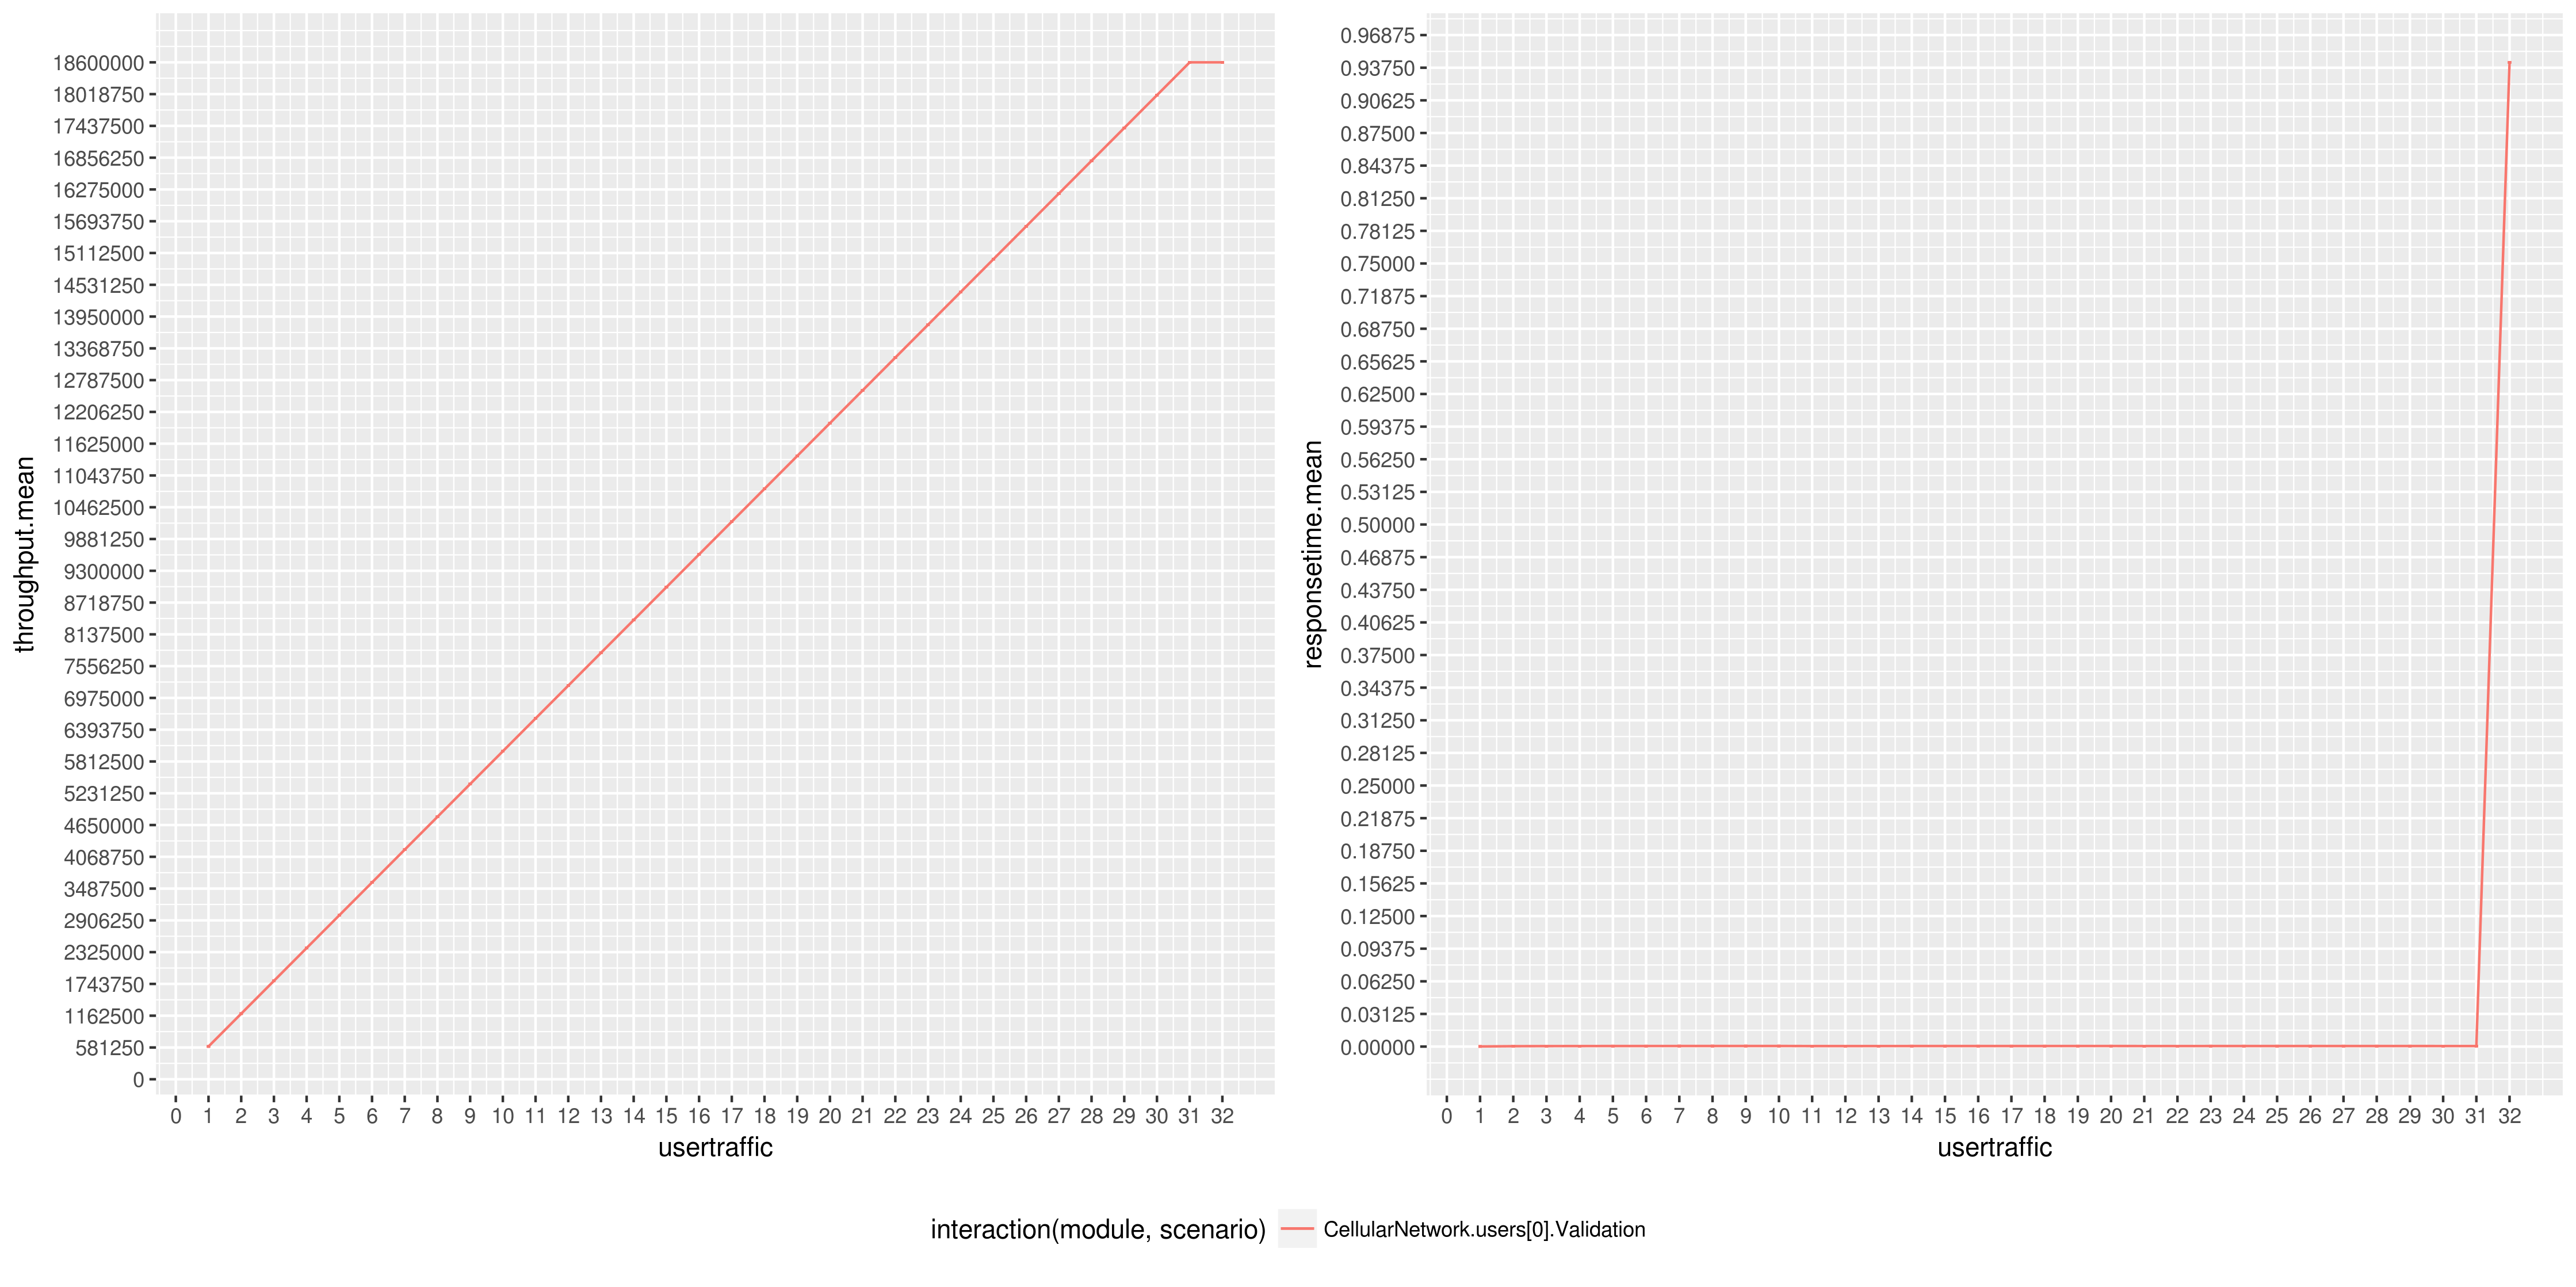
\includegraphics[width=1\textwidth]{images/plotvalidation}
  \caption{1st validation scenario: throughput, response time}
  \label{fig:1st validation scenario: throughput, response time}
\end{figure}

\section{2\textsuperscript{nd} test: fixed CQI, fixed \(\lambda\) rate, fixed packet size, 2 users}
In this test there are two \texttt{Mobile Stations} connected to antenna. As in the previous scenario all parameters are fixed. We have two indipendent flow of data from \texttt{Web Servers} to \texttt{Antenna} so the input throughtput could by computed as
\begin{equation} 
th\textsubscript{in} = \frac{packetsize\textsubscript{0} \times 8}{1/(1000\lambda\textsubscript{0})} + \frac{packetsize\textsubscript{1} \times 8}{1/(1000\lambda\textsubscript{1})}
\end{equation}
For these simulation we have chosen the following parameters:
\begin{itemize}
	\item \(packetsize_{0} = packetsize_{1} = 40\)
	\item \(CQI_{0} = 6\)
	\item \(CQI_{1} = 15\)
	\item \(\lambda = \lambda_{0} = \lambda_{1}\) and \(\lambda \in \{1,2,\ldots,32\}\)
\end{itemize}
We can compute the max \textit{slotted thorughput} for both users.
\begin{equation}
	\begin{split}
	slotth^{0}_{out} &= \frac{\#RB \times RBsize_{0} \times 8 }{T_s} = \frac{25 \times 20 \times 8}{0.001} = 4 \textnormal{ Mbps} \\ 
	slotth^{1}_{out} &= \frac{\#RB \times RBsize_{1} \times 8 }{T_s} = \frac{25 \times 93 \times 8}{0.001} = 18.6 \textnormal{ Mbps}
	\end{split}
\end{equation} 
\begin{figure}[H]
  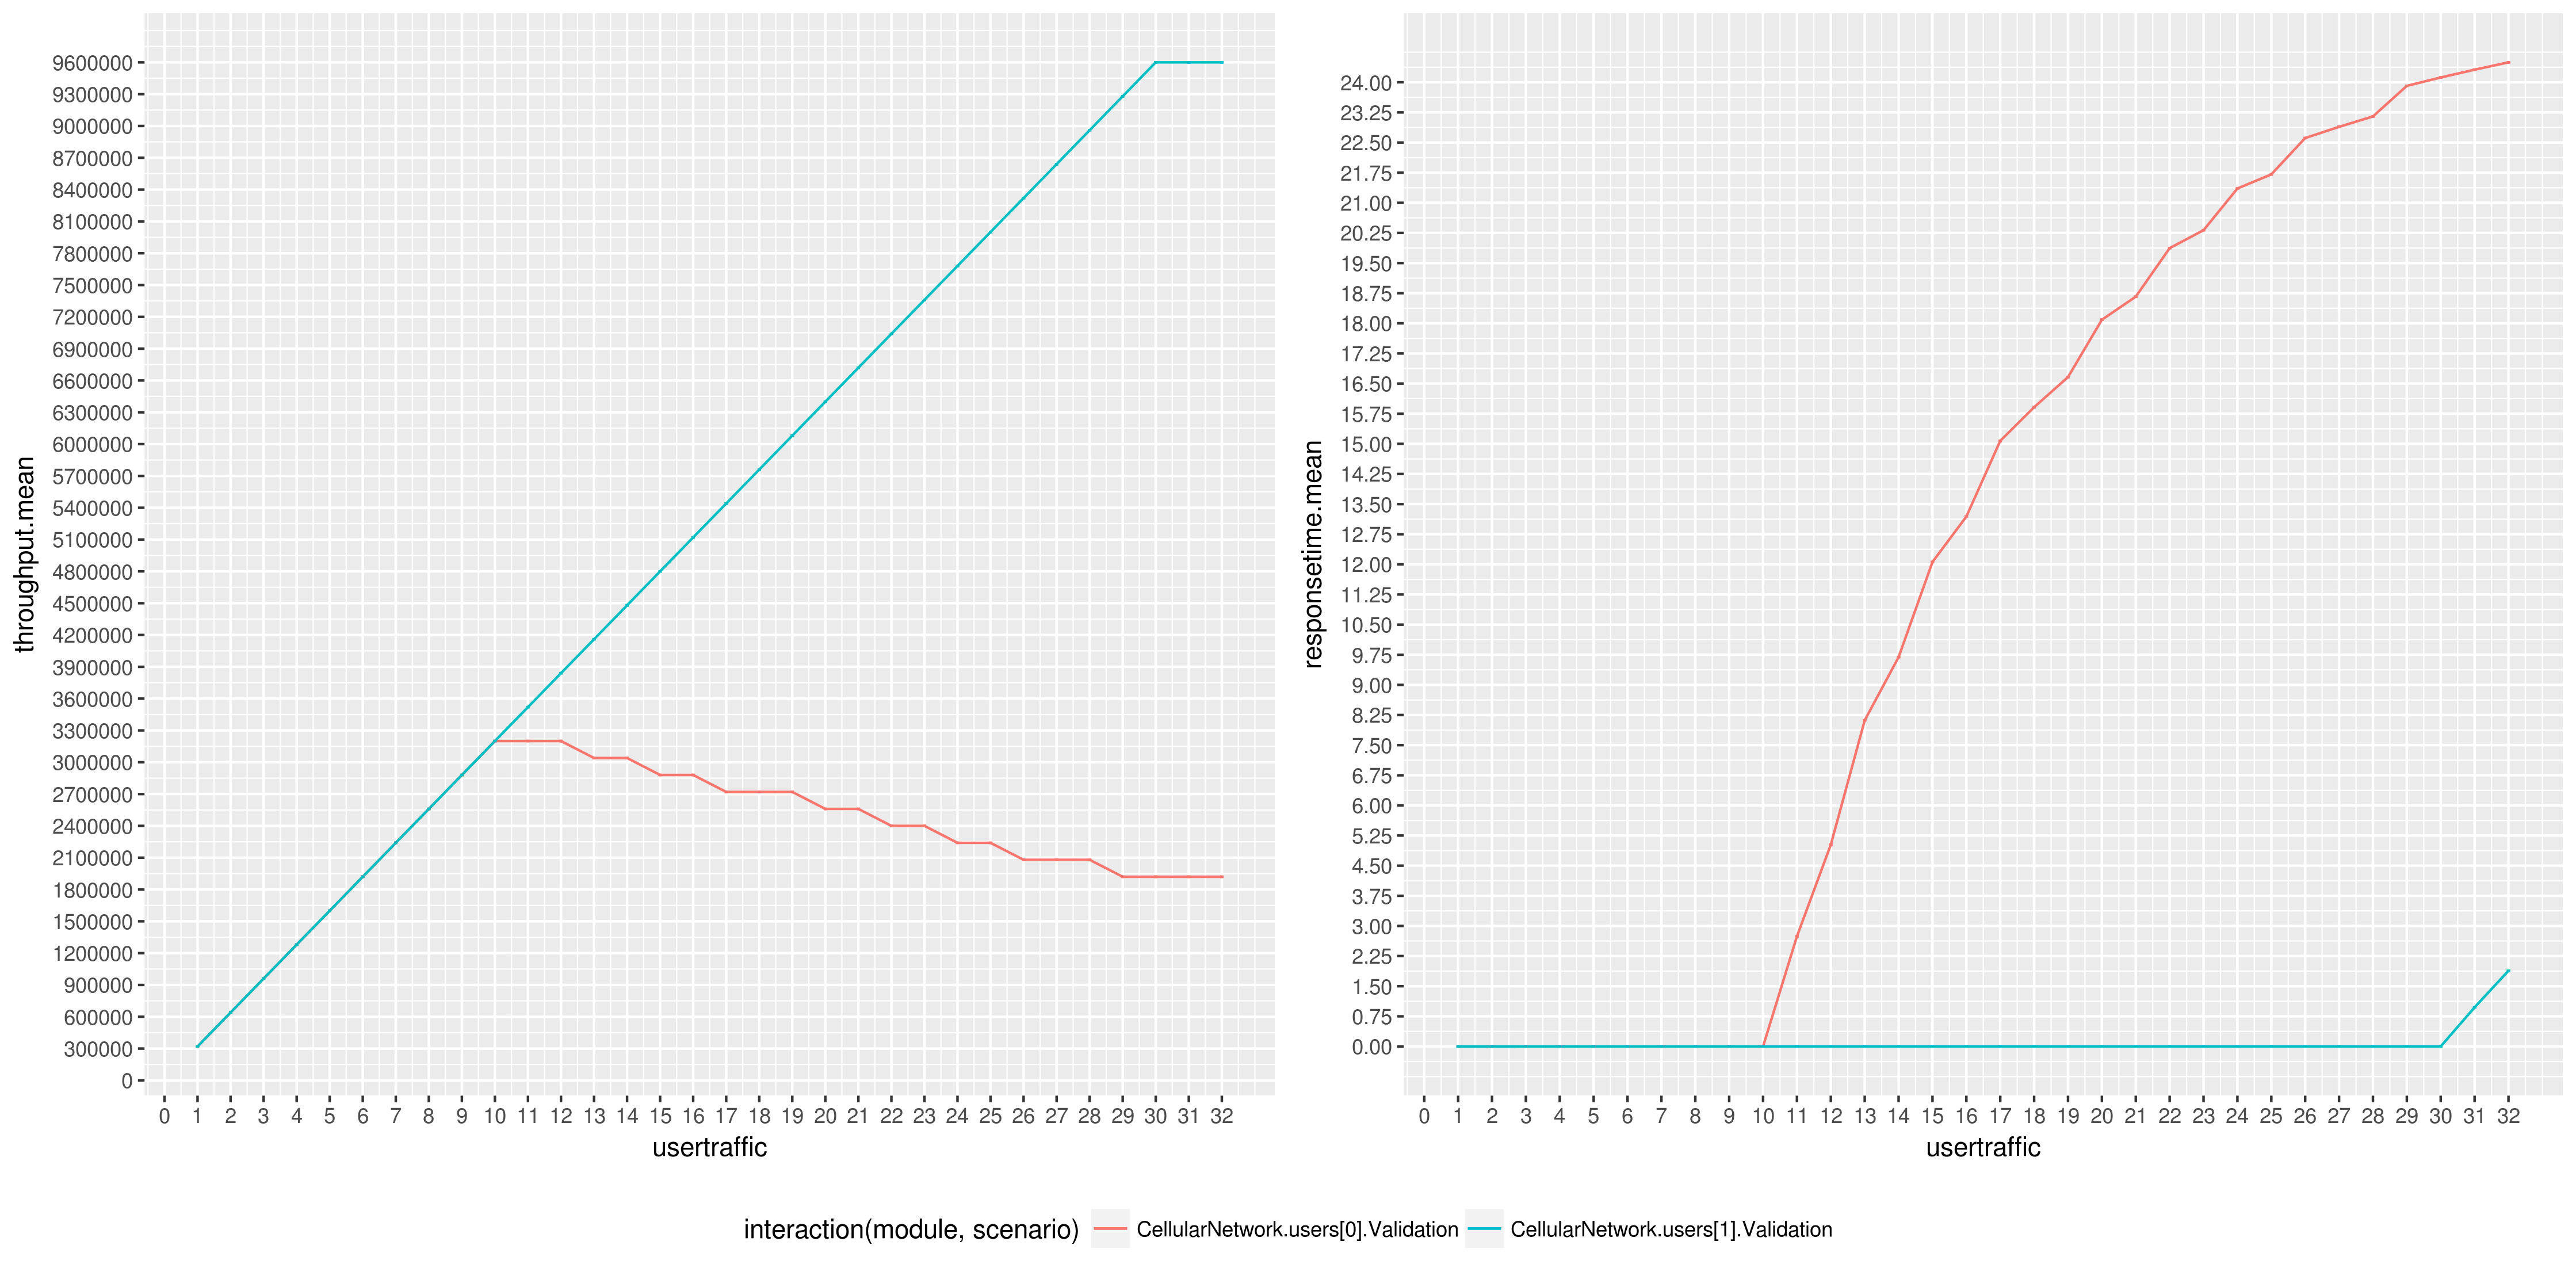
\includegraphics[width=1\textwidth]{images/plotvalidation2}
  \caption{2nd validation scenario: throughput, response time}
  \label{fig:2nd validation scenario: throughput, response time}
\end{figure}
At full load we expect that users compete to fill the frame. If the scheduler were fair, at full load, the average throughput would be \(th^{i}_{out} = (slotth^{i}_{out})/2\) since there are 2 users and the scheduler follow a round robin scheme, which is fair in principle. 

We see in the graph that throghput grows linear ad is equal for both users when \(1 \leq \lambda \leq 10 \). For \(\lambda > 10 \) the \texttt{Mobile User[0]} saturates, conversely \texttt{Mobile User[1]} continues to increase its throughput until it reaches saturation at \(\lambda = 30\).
When \(\lambda = 10 \) the input flow is \(th_{in}^{0} = th_{in}^{1} = (40 \times 8)/0.0001 = 3.2\textnormal{ Mbps}\) and this result could be seen also in the graph. Infact when \(\lambda \le 10 \) both users are in stable state so \(th_{in} = th_{out}\). We can see that, when \(\lambda\) increases the mean throughput approches to the half of slotted throughput as said before. However there is a small difference between the expected mean throughput and the result of simulation. This oddity can be explained better by analyzing the following graph, which shows the mean resource block per frame assigned to users.
\begin{figure}[H]
  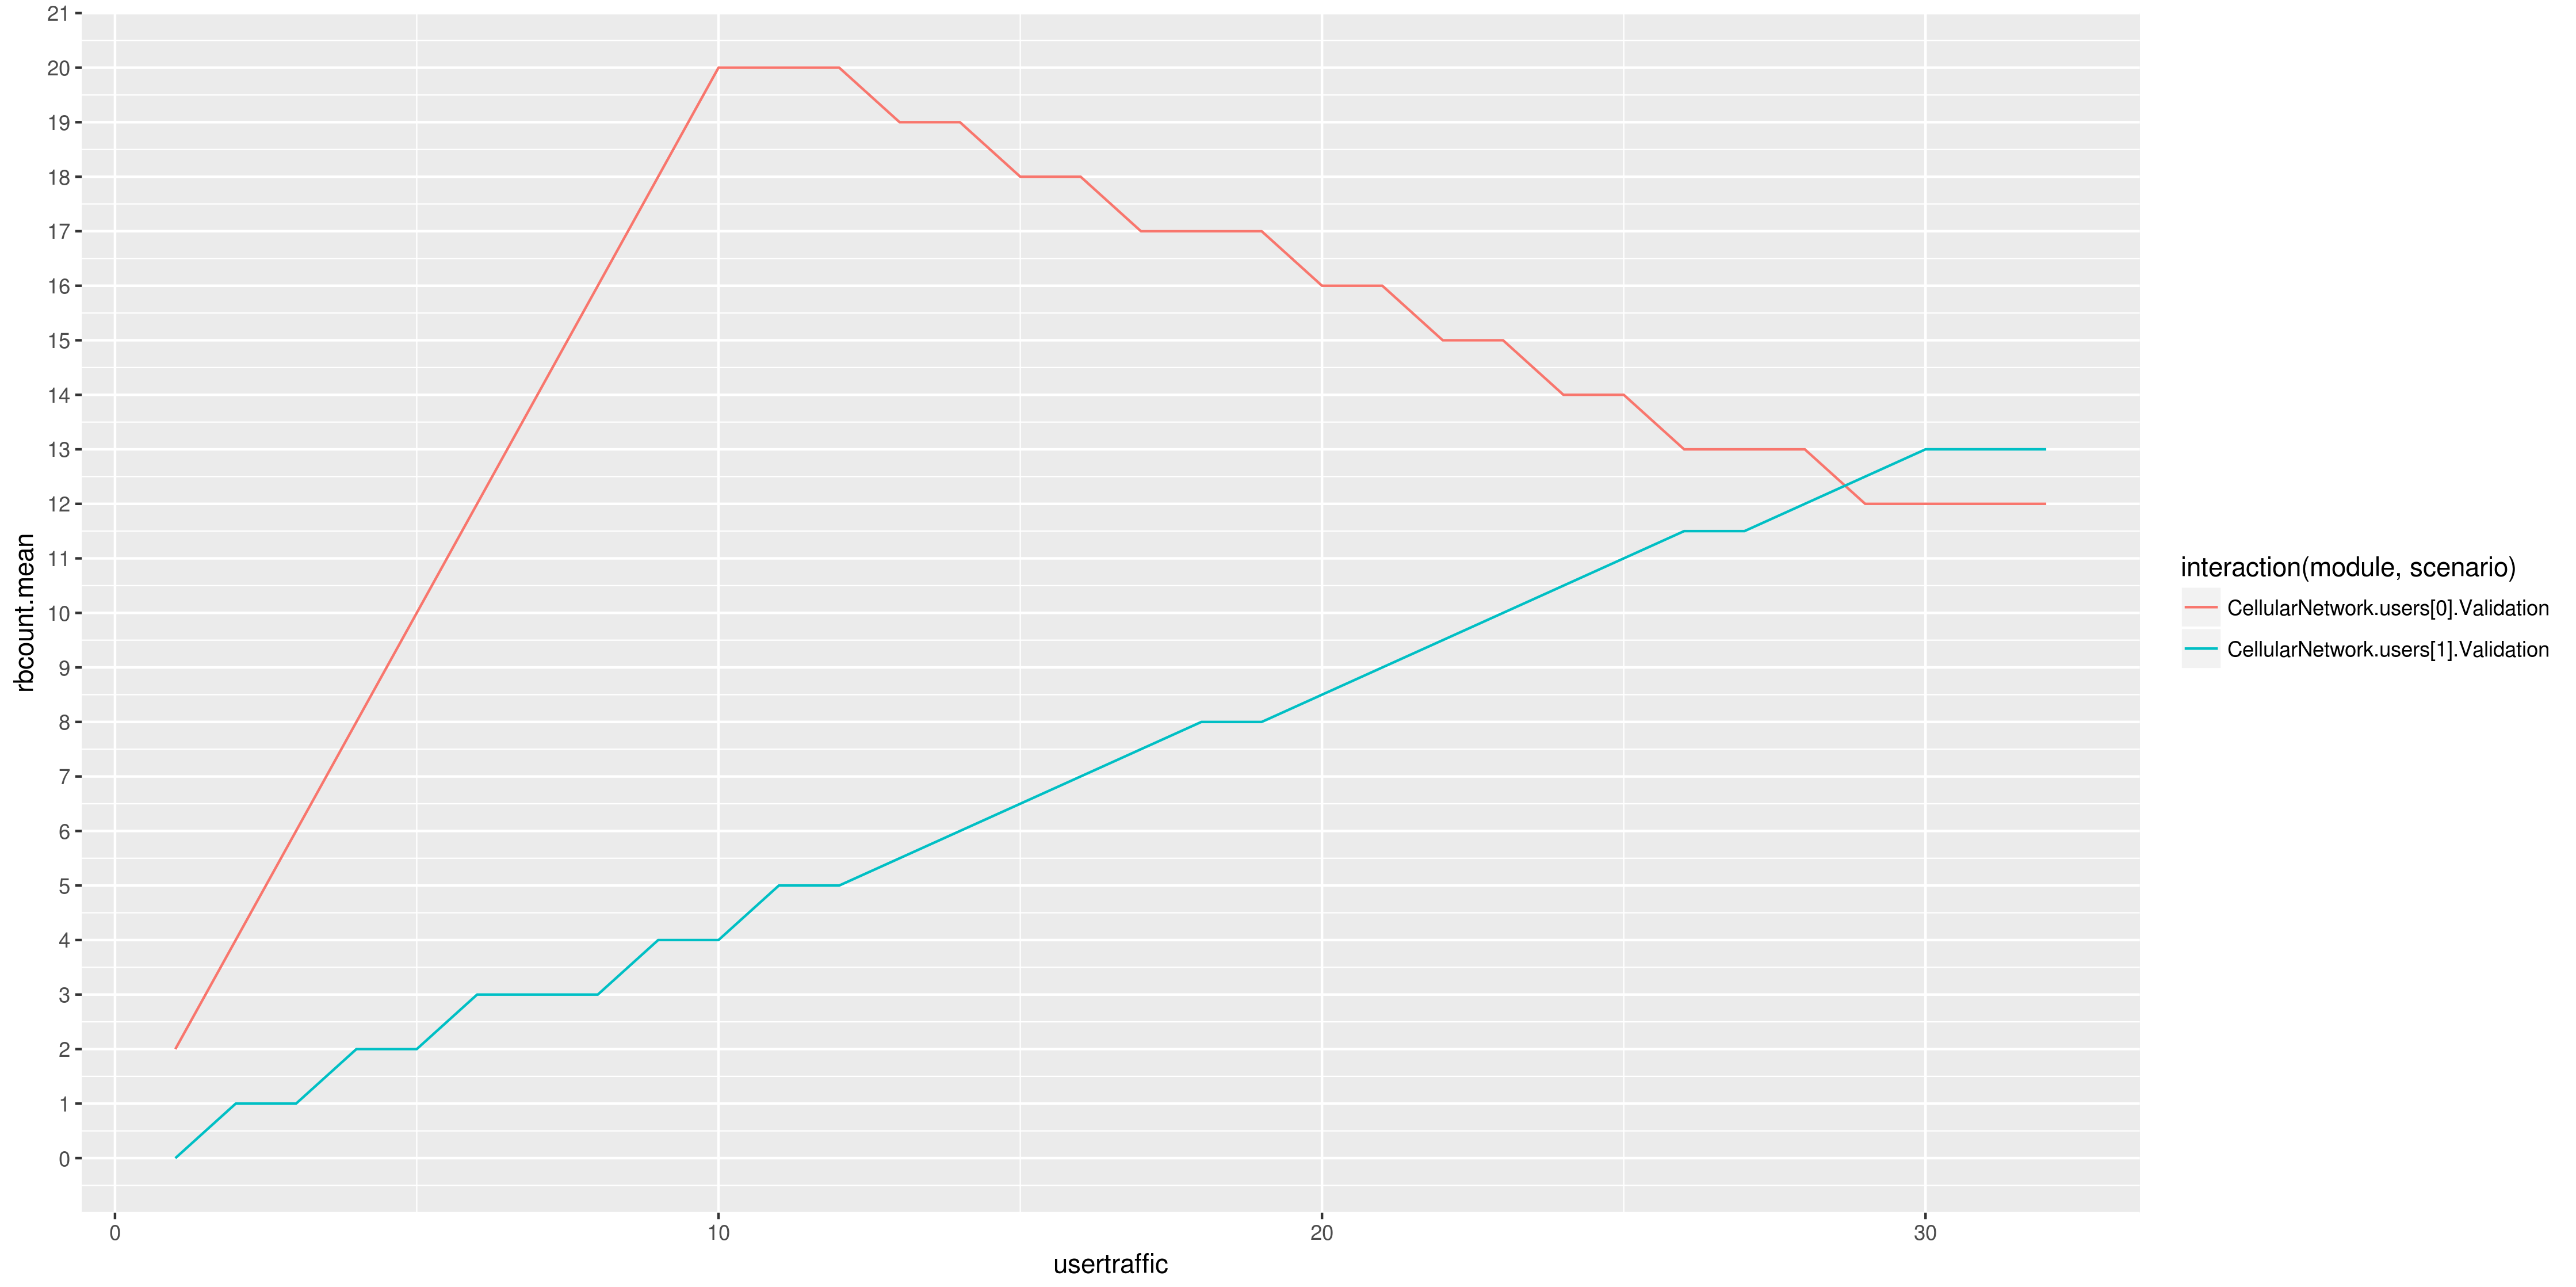
\includegraphics[width=1\textwidth]{images/RBCompvalidation2}
  \caption{2nd validation scenario: mean RB count}
  \label{fig:2nd validation scenario: mean RB count}
\end{figure}
By math the mean RB would be \(\#RB / 2 = 12.5 \) but the number of RB assigned per user is slightly different since, on average, 11 RBs are assigned to \texttt{Mobile User[0]} and 13 RBs are assigned to \texttt{Mobile User[1]}. This oddness is due to fragmentation of packet. In our simple model infact packets can not be fragmented so if a packet does not fill inside the last RB this RB is lost and it assigned to the next user. Note that in validation scenarios everything is fixed, also packet dimension, so there could be strangeness like that. However we can say that our model is quite accurate and can be used to simulate the network in more complex scenarios. 
There is another strange behavior that involves response time. When the input traffic is too high we expect that response grows indefinitely since packets get queued. However, by observing the graph, the mean response time seems to approch to \(ST/2\). In the following graph it is displayed the response time of packets addressed to \texttt{Mobile Station[0]} when the rate \(\lambda = 40\), so it is very high.
\begin{figure}[H]
  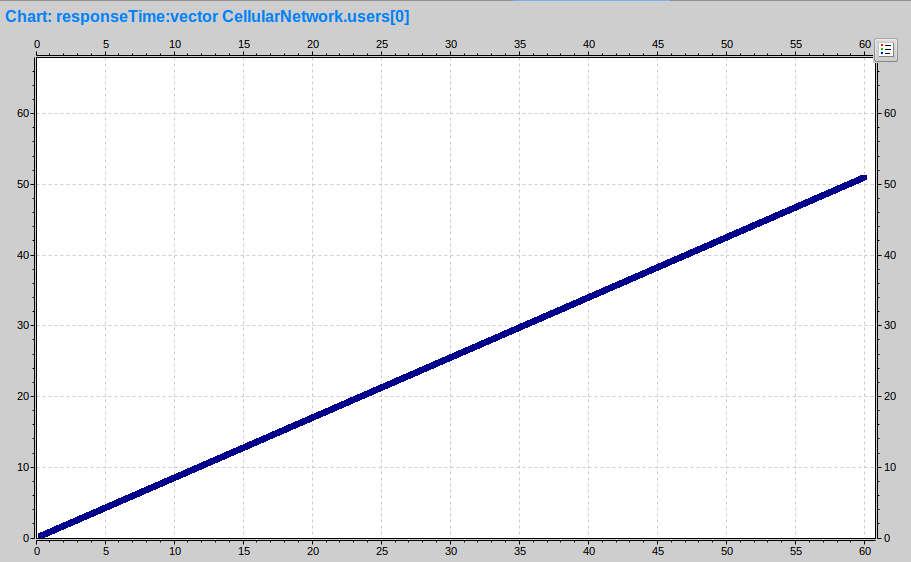
\includegraphics[width=1\textwidth]{images/response-timeVec}
  \caption{2nd validation scenario: response time(vector)}
  \label{fig:2nd validation scenario: response time(vector)}
\end{figure}
We we can see cleary a linear relation between simulation time and response time when the system is unstable. We can describe the relation as:
\begin{equation} 
	RT(t) \approx \frac{\max(RT)}{ST}t, \quad 0\le t \le ST 
\end{equation}
The previous formula has that meaning: \textit{a packet which is generated at time t will have a response time about equal to \(RT(t)\)}. Now we can try to calculate the \textit{mean response time}.
\begin{equation}
\begin{split}
E[RT(ST)] &= \frac{\sum\limits^{ST}_{t=0} RT(t)}{ST} = \frac{\sum\limits^{ST}_{t=0} \frac{\max(RT)}{ST}t}{ST} = \frac{\max(RT)}{ST^2}\sum\limits^{ST}_{t=0}t =
	\\ &= \frac{\max(RT)}{ST^2}\frac{ST(ST+1)}{2} = \frac{\max(RT)}{2}\frac{ST+1}{ST} \approx \frac{\max(RT)}{2}
\end{split}
\end{equation}
At the end we can observe that if the system is unstable \(RT(t)\) has a linear behavior so if we calculate the mean at the end of simulation we obtain \(E[RT(ST)] \approx ST/2\). 


\section{3\textsuperscript{rd} test: NoFramingTest, uniform CQI, exponential interarrivals, fixed packet size, 10 users}

This is a test to validate eventually the model shown in the previous chapter. It's too difficult to build a full matematical model starting from the requirements, but having no one is not helpful in explaining the simulation results. So we started to build simple models by leaving off some of the requirements and by considering only some specific conditions (like saturation). In our case one of the most difficult things to model is packet framing: as the requirements said, every RB cannot contain packets from two or more different users. This means that there will be some wasted space to consider. Furthermore, if a packet cannot completely fill the frame, it cannot be scheduled and the scheduler moves to the next user.

A question now arises: how this packet framing policy will influence our results? Intuition make us think that total antenna throughput will get somewhat worse, just thinking about the wasted space.
To confirm this intuition we set up another scenario, called NoFramingTest, which will be running using the following parameters:

\begin{itemize}
	\item \(\#users = 10\)
	\item \(CQI_i \sim U(1,15)\)
	\item \(packetsize_i=25 \textnormal{ B}\)
	\item \(interarrivalrate_i \sim exp(\lambda)\)
\end{itemize}

The most strange parameter here is \(packetsize\). This is a simple way to have no framing at all in our simulation. We could end up fixing \(packetsize=1 \textnormal{ B}\), which would be the simplest way, however simulation would be too heavy to run at higher traffic rates (we tried, but our PCs started frying). Recalling that we need just to check throughput in saturation, we can suppose that every frame is only filled with packets from the currently selected user (using RR policy).
Studying the formula that defines the total frame size of each client in our model:
\begin{equation}
	\begin{split}
	&rbsize_i = f(CQI_i) \\
	&framesize_i = \#RB \times rbsize_i
	\end{split}
\end{equation}
The number of packets that will fill the frame can be computed as:
\begin{equation}
\#packets_i = framesize_i/packetsize
\end{equation}
where \(packetsize\) is fixed, our goal is to find a \(packetsize\) such that \(\#packets_i\) is a natural number (all packets fill exactly the frame) for each client (\(i\)).
As we said, \(packetsize=1\) is a solution, however another interesting solution is \(packetsize=25\). This is due to the fact the \(\#RB=25\) is fixed and used to compute every client frame size. Note that this is valid only if frame is filled every time by a single client (as the previous assumption). Lets check the results:

\begin{center}
	INSERIRE GRAFICO THANTENNA QUI\\
	INSERIRE GRAFICO FILLRB QUI\\
	(dovrebbe essere esattamente a zero quando i client saturano)
\end{center}

A simple mathematical model to compute antenna total throughput can be:
\begin{equation}
	E[th_{antenna}] = \frac{\sum\limits_{i=1}^{\#client} \#RB \times E[rbsize_i]}{\#client\times(1/T_{slot})} = \frac{\sum\limits_{i=1}^{10} 25 \times E[rbsize_i]}{10 \times (1/T_{slot})}
\end{equation}
\(rbsize_i\) is a RV variable with an unknown distribution, however
\begin{equation}
	 rbsize_i = f(CQI_i), \quad CQI_i\sim U(1,15), \quad \forall i \in [1,10]
\end{equation}
This means we can simply use the general formula for functions of RVs
\begin{equation}
	E[X] = \sum_{x_i : g(x_i)=y_i}^{} g(x)p(x) = E[g(x)]
\end{equation}
Considering that
\[f(CQI_i) = [3,3,6,11,15,20,25,36,39,50,63,72,80,93,93] \]
our result, that will be used also in other computations, is
\begin{equation}
	E[rbsize_i] = \frac{1}{15} \times \sum_{i=1}^{10} f(CQI_i) =40.6 \textnormal{ B}, \quad \forall i \in [1,10]
\end{equation}
which is constant for all clients. In this case the initial model can be simplified to
\begin{equation}
E[th_{antenna}] = \frac{\#RB \times E[rbsize_i]}{1/T_{slot}} \times 8 = 8.12 \textnormal{ Mbps}
\end{equation}
The mean \textbf{matches exactly} the simulation results!

This test is not only for a validation purpose, but it is a starting point to study how fragmentation impacts network performances. We will see this later.